\section{Project description}
%% \begin{frame}{Grasp of thin objects}
%%   \begin{columns}
%%     \begin{column}{0.5\textwidth}
%%       \includemedia[
%%         activate=pageopen,
%%         width=160pt,height=90pt,
%%         addresource=videos/hand_fail.mp4,
%%         flashvars={%
%%           src=videos/hand_fail.mp4
%%           &scaleMode=stretch&autoPlay=true&loop=true
%%           &hideBar=true}
%%       ]{}{StrobeMediaPlayback.swf}
%%     \end{column}
%%     \begin{column}{0.5\textwidth}
%%       \begin{alertblock}{Problem}
%%         Performing the grasp of thin objects could be a hard task
%%         because not enough contact constraints are provided by the object
%%       \end{alertblock}
%%     \end{column}
%%   \end{columns}
%% \end{frame}

\begin{frame}{Grasp of thin objects}
  \vskip 0.1in
    \begin{alertblock}{Problem}
      Performing the grasp of thin objects could be a hard task
      because not enough contact constraints are provided by the object
    \end{alertblock}
    \begin{center}
      \includemedia[
        activate=pageopen,
        width=285.3pt,height=158.85pt,
        addresource=videos/hand_fail.mp4,
        flashvars={%
          src=videos/hand_fail.mp4
          &scaleMode=stretch&autoPlay=true&loop=true
          &hideBar=true}
      ]{}{StrobeMediaPlayback.swf}
    \end{center}
\end{frame}


\begin{frame}{A solution to the problem}
  Use of environmental constraints to arrange an easier grasp and
  then perform the grasp
  \begin{columns}
    \begin{column}{0.5\textwidth}
      \vskip+0.1in
      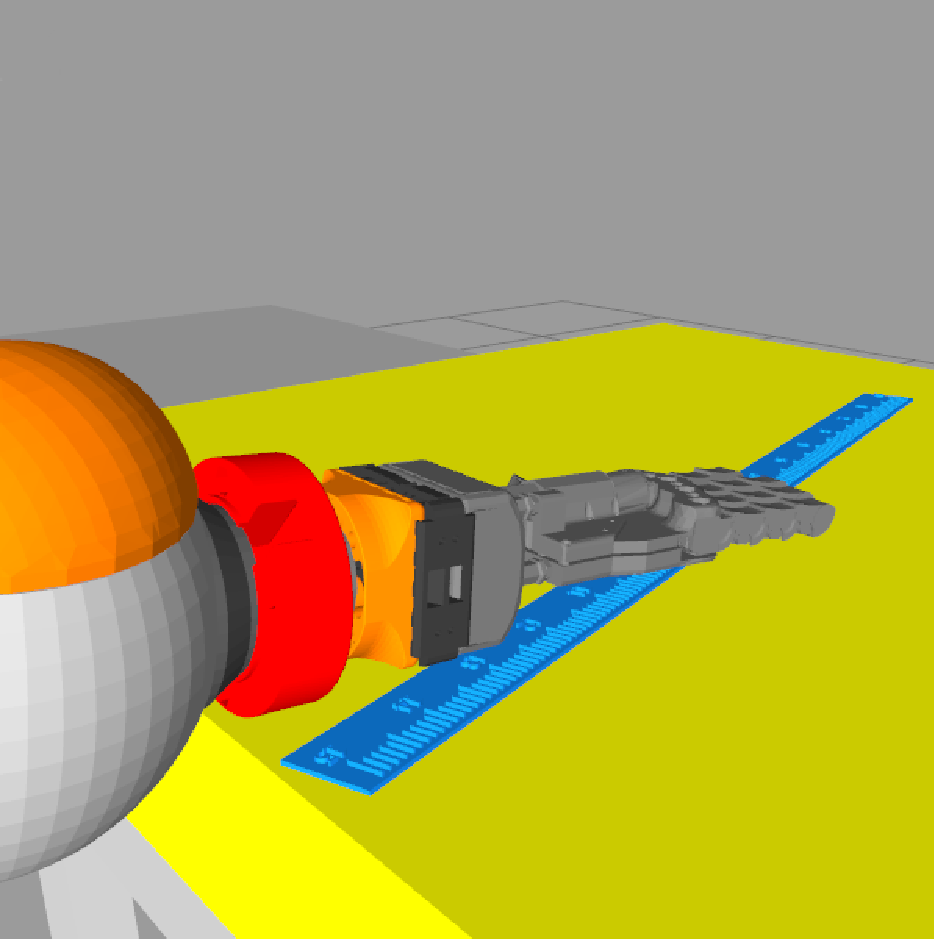
\includegraphics[width=\columnwidth]{hand_on_ruler}
    \end{column}
    \begin{column}{0.5\textwidth}
      \begin{exampleblock}{Example}
        \begin{itemize}
        \item[1.] the hand is placed on the object
        \item[2.] the hand drags the object until it \alert{sticks out 
          of the border} of the table 
        \item[3.] the hand grasps the object
        \end{itemize}
      \end{exampleblock}
    \end{column}
  \end{columns}
\end{frame}

\begin{frame}{How to perform a safe dragging phase}
  The dragging phase could \alert{damage} the object due to uncontrolled contact forces between the 
  hand and the object.
  \par
  An hybrid position force control strategy allows to avoid this issue.
  \vskip0.5in
  \begin{exampleblock}{Aim of this project}
    Develop an hybrid force position control that allows to move the hand and 
    at the same time to regulate the contact force using a force feedback signal.
  \end{exampleblock}
\end{frame}

\begin{frame}{Control architecture}
  The hybrid force position control was obtained using the \alert{Hybrid Impedance Approach (HIC)}
  proposed by Anderson and Spong in the $1988$.
  \par 
  This approach requires the existence of an \alert{inverse dynamics} control \alert{inner} loop
  to cancel the nonlinearities of the manipulator 
  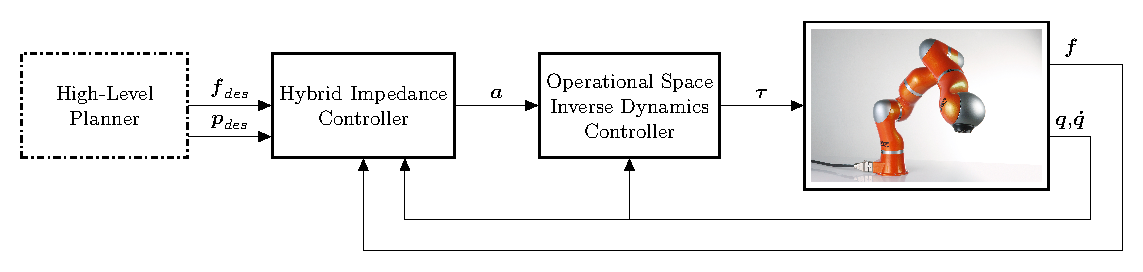
\includegraphics[width=\columnwidth]{control_arch}
  \par
  The inner loop applied to the manipulator results in a double integrator system
  $\ddot{\vec{x}} = \vec{a}$ where $\vec{x}$ is a Cartesian description of the end-effector
  and $\vec{a}$ is chosen using the HIC approach.
\end{frame}

\begin{frame}{Contents}
  The contents presented are
  \begin{itemize}
  \item[-] the HIC approach
  \item[-] the development of a HIC based outer control loop
  \item[-] the inverse dynamics inner loop
  \item[-] how to correctly use a force torque sensor that is required to close the outer loop
  \item[-] the results obtained in simulation and in a real scenario
  \item[-] notes about the software implementation
  \item[-] future works
  \end{itemize}
\end{frame}

